%=====================================================================
%  MMSS Graph Theory  .  Daily Report + Solutions Template
%
%  How to use:
%    1. Rename per session, e.g. mmss_graphtheory_0722.tex
%    2. Edit the two \newcommand lines just below (team + date).
%    3. Edit the FRONTMATTER block inside the document.
%    4. Write problems inside the enumerate. Use the graph toolkit.
%
%  Graph toolkit cheat sheet (all go INSIDE a graphfig / tikzpicture):
%    \gcycle{n}{radius}{prefix}      n vertices on a circle, joined as a cycle
%    \gcyclen{n}{radius}{prefix}     same, but vertices numbered 1..n
%    \gcomplete{n}{radius}{prefix}   complete graph K_n on a circle
%    \gbipartite{m}{n}{gap}          complete bipartite K_{m,n} (nodes bl1.., br1..)
%    \gpath{n}{spacing}{prefix}      path on n vertices, left to right
%    \gpeterson                      the Petersen graph
%    \gcube{n}                       n x n x n cube in oblique 2D projection
%  Vertex styles:  v (filled dot)  .  ov (open ring)  .  hv (highlighted hub)
%  Figure wrapper:  \begin{graphfig}[scale]{Label} ... \end{graphfig}
%=====================================================================
\documentclass[11pt]{article}

\usepackage[margin=1in,headheight=30pt,headsep=16pt]{geometry}
\usepackage{amsmath,amssymb,amsfonts,amsthm,xcolor}
\usepackage{enumitem}
\usepackage{fancyhdr}
\usepackage{graphicx}
\usepackage{tikz}
\usepackage{xcolor}
\usetikzlibrary{arrows.meta,calc}
\newcounter{mycounter}
\stepcounter{mycounter}



\newcommand{\teamname}{GROUP NAME}
\newcommand{\reportdate}{\today}


\pagestyle{fancy}
\fancyhf{}
\renewcommand{\headrulewidth}{0.4pt}
\renewcommand{\footrulewidth}{0pt}
\fancyhead[L]{\raisebox{2pt}{\small\textsc{\teamname}}}
\fancyhead[R]{
\includegraphics[height=10pt]{image.png}}   
\fancyfoot[C]{\small\thepage}


\fancypagestyle{firstpage}{
  \fancyhf{}
  \renewcommand{\headrulewidth}{0pt}
  \fancyfoot[C]{\small\thepage}
}

\setlength{\parindent}{0pt}
\setlength{\parskip}{6pt}


\newcommand{\divider}{\begin{center}\rule{0.6\textwidth}{0.4pt}\end{center}}


\newtheoremstyle{solstyle}{6pt}{6pt}{}{}{\bfseries}{.}{ }{}
\theoremstyle{solstyle}
\newtheorem*{solution}{Solution}


\newcommand{\WLoG}{WLoG}
\newcommand{\Cn}[1]{C_{#1}}
\newcommand{\Kn}[1]{K_{#1}}
\newcommand{\Kt}[2]{K_{#1,#2}}
\tikzset{
  v/.style ={circle, fill=black, inner sep=1.6pt},
  ov/.style={circle, draw=black, fill=white, line width=0.6pt, inner sep=1.6pt},
  hv/.style={circle, fill=black!55, draw=black, line width=0.6pt, inner sep=2.6pt},
  edge/.style={line width=0.6pt},
}

\newcommand{\gcycle}[3]{
  \foreach \gi in {1,...,#1}{\node[v] (#3\gi) at ({90-(\gi-1)*360/#1}:#2){};}
  \foreach \gi in {1,...,#1}{\pgfmathtruncatemacro{\gj}{mod(\gi,#1)+1}\draw[edge] (#3\gi)--(#3\gj);}
}

\newcommand{\gcyclen}[3]{
  \foreach \gi in {1,...,#1}{
    \pgfmathsetmacro{\gang}{90-(\gi-1)*360/#1}
    \node[v,label={\gang:\gi}] (#3\gi) at (\gang:#2){};}
  \foreach \gi in {1,...,#1}{\pgfmathtruncatemacro{\gj}{mod(\gi,#1)+1}\draw[edge] (#3\gi)--(#3\gj);}
}

\newcommand{\gcomplete}[3]{
  \foreach \gi in {1,...,#1}{\node[v] (#3\gi) at ({90-(\gi-1)*360/#1}:#2){};}
  \foreach \gi in {1,...,#1}{\foreach \gj in {1,...,#1}{\ifnum\gi<\gj\relax\draw[edge] (#3\gi)--(#3\gj);\fi}}
}

\newcommand{\gbipartite}[3]{
  \foreach \gi in {1,...,#1}{\node[v] (bl\gi) at (0,{(#1+1)/2-\gi}){};}
  \foreach \gj in {1,...,#2}{\node[v] (br\gj) at (#3,{(#2+1)/2-\gj}){};}
  \foreach \gi in {1,...,#1}{\foreach \gj in {1,...,#2}{\draw[edge] (bl\gi)--(br\gj);}}
}

\newcommand{\gpath}[3]{
  \foreach \gi in {1,...,#1}{\node[v] (#3\gi) at ({(\gi-1)*#2},0){};}
  \pgfmathtruncatemacro{\gplast}{#1-1}
  \foreach \gi in {1,...,\gplast}{\pgfmathtruncatemacro{\gpk}{\gi+1}\draw[edge] (#3\gi)--(#3\gpk);}
}

\newcommand{\gpeterson}{
  \foreach \pi in {0,...,4}{
    \node[v] (po\pi) at ({90+\pi*72}:2){};
    \node[v] (pin\pi) at ({90+\pi*72}:1){};}
  \foreach \pi in {0,...,4}{
    \pgfmathtruncatemacro{\pj}{mod(\pi+1,5)}
    \pgfmathtruncatemacro{\pk}{mod(\pi+2,5)}
    \draw[edge] (po\pi)--(po\pj);
    \draw[edge] (po\pi)--(pin\pi);
    \draw[edge] (pin\pi)--(pin\pk);
  }
}


\newcommand{\qgon}[2]{
  \pgfmathtruncatemacro{\Nm}{2^#1-1}
  \pgfmathtruncatemacro{\nm}{#1-1}
  \foreach \i in {0,...,\Nm}{
    \pgfmathsetmacro{\ang}{90-\i*360/(\Nm+1)}
    \xdef\lbl{}
    \foreach \k in {\nm,...,0}{
      \pgfmathtruncatemacro{\bit}{mod(floor(\i/(2^\k)),2)}
      \xdef\lbl{\lbl\bit}
    }
    \node[v,label={\ang:\scriptsize $\lbl$}] (q\i) at (\ang:#2){};
  }
  \foreach \i in {0,...,\Nm}{
    \foreach \k in {0,...,\nm}{
      \pgfmathtruncatemacro{\bit}{mod(floor(\i/(2^\k)),2)}
      \ifnum\bit=0
        \pgfmathtruncatemacro{\j}{\i+2^\k}
        \draw[edge] (q\i)--(q\j);
      \fi
    }
  }
}
\newcommand{\gcube}[1]{
  \begin{scope}[x={(1cm,0cm)}, y={(0cm,1cm)}, z={(0.5cm,0.45cm)}]
    \foreach \ci in {0,...,#1}{\draw[edge] (\ci,0,0)--(\ci,#1,0);}  
    \foreach \cj in {0,...,#1}{\draw[edge] (0,\cj,0)--(#1,\cj,0);}
    \foreach \ci in {0,...,#1}{\draw[edge] (\ci,#1,0)--(\ci,#1,#1);} 
    \foreach \ck in {0,...,#1}{\draw[edge] (0,#1,\ck)--(#1,#1,\ck);}
    \foreach \cj in {0,...,#1}{\draw[edge] (#1,\cj,0)--(#1,\cj,#1);} 
    \foreach \ck in {0,...,#1}{\draw[edge] (#1,0,\ck)--(#1,#1,\ck);}
    \foreach \ci in {0,...,#1}{\foreach \cj in {0,...,#1}{\node[v] at (\ci,\cj,0){};}}
    \foreach \ci in {0,...,#1}{\foreach \ck in {0,...,#1}{\node[v] at (\ci,#1,\ck){};}}
    \foreach \cj in {0,...,#1}{\foreach \ck in {0,...,#1}{\node[v] at (#1,\cj,\ck){};}}
  \end{scope}
}
\newenvironment{graphfig}[2][1]{
  \def\gflabel{#2}
  \begin{tabular}{@{}c@{}}
  \begin{tikzpicture}[scale=#1]
}{
  \end{tikzpicture}
  \ifx\gflabel\empty\else\\[3pt]\textbf{[Graph \gflabel]}\fi
  \end{tabular}
}

\newcommand{\glabel}[1]{\begin{center}\textbf{[Graph #1]}\end{center}}
\begin{document}
\thispagestyle{firstpage}
\noindent\textbf{\teamname}\hfill\textbf{\reportdate}

\noindent\textbf{Clarifier:} Changhwan\\
\textbf{Manager:} Benjamin\\
\textbf{Reporter:} Sharan\\
\textbf{Skeptic:} Henry


%instructor palettes
\definecolor{INSTRUCTOR0}{HTML}{FF0000}
\definecolor{INSTRUCTOR1}{HTML}{00FF00}
\definecolor{INSTRUCTOR2}{HTML}{0000FF}

\color{blue} Rachel is Blue . 
\color{black}

\textbf{Report:} Our group worked well together today, splitting the homework problems to solve efficiently and helping each other when needed. Specifically, we were able to solve questions $2, 3, 5, 6, 8, 9 \text{ and } 10$ somewhat easily, though we found questions $1 \text{ and } 4$ to be particularly difficult. For many of the questions involving proof or disproof, we tried numerous counter-examples that turned out to have very easy problems. For example, in question 1, we came up with numerous graphs that had cycles that did not have chords, but didn't seem obvious to see. Another problem we had was with proper collaboration - everyone was everywhere, and in the future we should probably discuss problems a bit longer together.

\divider

\textbf{SOLUTIONS \& PROOFS:}\\
Without Loss of Generality is abbreviated as \WLoG{} within this document.
\color{red} You really don't need a macro for WLoG lol \color{black} \color{green}Definition of a computer scientist: Someone who will spend 3 hours figuring out a way to save 15 seconds next time. I approve\color{black}

\begin{enumerate}[leftmargin=*]

\item We proved that all interval graphs were chordal. Prove that not all chordal graphs are interval graphs. 
    \begin{proof}Counterexample. 
    \begin{center}
        \begin{graphfig}{\themycounter\stepcounter{mycounter}}
            \gcycle{5}{0.9}{a}
            \draw (a1)--(a4) (a2)--(a5) (a3)--(a5);
        \end{graphfig}
    \end{center}
    \end{proof}\color{red} Not chordal; has a 4-cycle with no chord. \color{black}
\item A forest is an acyclic graph. 
\begin{enumerate}
    \item Why do you think such a graph is called a forest? 
        
    \begin{solution}
        Since there is no connected clause, we cannot call this graph itself a tree. However, if we split the forest into individual components, each are a \textbf{connected, acyclic graph}. Therefore, it is a \textbf{cluster of tress}, a forest. 
    \end{solution}
    \item If a forest has order $n$ and $k$ components, how many edges does it have? 
    \begin{solution}
        $n-k$
    \end{solution}
    \begin{proof}
        Let the forest be split into $k$ trees. Let each tree have $v_i$ verticies. By the alternate definition of the tree, each tree has $v_i-1$ edges. If we sum this up, we get
        $$ \sum_{i=1}^k v_i-1 = \sum_{i=1}^k v_i - \sum_{i=1}^k 1 = n - k $$
    \end{proof} \color{red} Great! \color{black}
\end{enumerate}
\item Prove or disprove : Every graph with fewer edges than vertices has at least on component that is a tree. 
\begin{solution}
    Proved. 
\end{solution}
\begin{proof}
    Suppose not. Say we have a graph with fewer edges($m$) than vertices($n$) without a tree. Say the graph is partitioned into $k$ components, each with $v_i$ vertices. Let us try to force each component to \textit{not} be a tree. Since each component has to be connected and not a tree, each component needs a minimum of $v_i$ edges. Therefore, since the entire graph requires a minimum of $n$ edges, it goes against the initial claim that $m < n$. \color{red} Great! \color{black}
\end{proof}
\item Let $G$ be a graph with order $n$ and size $m$. Prove the following. 
\begin{enumerate}
    \item $G$ is a tree IFF $G$ is connected and acyclic. 
    \item $G$ is a tree IFF $G$ is connected and $m=n-1$. 
    \item $G$ is a tree IFF $G$ is acyclic, and if a single edge is added, it will have a cycle. 
    \item $G$ is a tree IFF there is a unique path between every pair of vertices in $G$. 
    \item $G$ is a tree IFF $G$ is connected and every edge of $G$ is a bridge. 
    \item $G$ is a tree IFF $G$ is acyclic and has exactly $n-1$ edges. 
\end{enumerate}
\item The $n$-cube (below written $Q_n$ is the graph whose vertex set is the set of all $n$ tuples of $0$s and $1$s. Examples : 
\begin{center}
$4$-tuples : 
\qquad
$0000$
\qquad
$0101$
\qquad
$1110$
\qquad
$1010$
\end{center}
\begin{center}
$7$-tuples : 
\qquad
$0111011$
\qquad
$1000111$
\qquad
$1010101$
\qquad
$1111111$
\end{center}
Two $n$ tuples are neighbors if they differ in precisely one coordinate. 
\begin{enumerate}
    \item Draw $Q_1$, $Q_2$, $Q_3$, and $Q_4$.
    \begin{solution}. 
    \begin{center}
    \begin{graphfig}{\themycounter\stepcounter{mycounter}}\qgon{1}{1}\end{graphfig}
    \begin{graphfig}{\themycounter\stepcounter{mycounter}}\qgon{2}{1.4}\end{graphfig}
    \begin{graphfig}{\themycounter\stepcounter{mycounter}}\qgon{3}{2}\end{graphfig}
    \begin{graphfig}{\themycounter\stepcounter{mycounter}}\qgon{4}{3.41}\end{graphfig}
    \end{center}
    \end{solution} \color{red} Didn't expect a macro for drawing $Q_n$! \color{black}

 \color{blue} This is a very satisfying layout for $Q_n$! \color{black}

    \item Prove $Q_n$ is regular.
    \begin{proof}
    For each vertices, we can relate with numbers by changing digits 0 to 1 or 1 to 0. Since we can change n tuples, the degree of each vertices are n which makes this graph n-regular. \color{red} Great! \color{black}
\end{proof}
    \item Prove $Q_n$ is bipartite. 
    \begin{proof}
    When we set A as vertices that has odd number of 1 and we set B as vertices that has even number of 1, we can have two set in the same number of vertices and see that this graph is bipartite. \color{red} This works as two independent sets; but this isn't what you've said here. You should be clearer about what these two sets have to do with each other, and why it shows the graph is bipartite. \color{black}
\end{proof}
\end{enumerate}
\item Prove $Q_n$ is Hamiltonian ( for $n > 1$)
\begin{proof}
    First of all this graph is bipartite. When we set A as vertices that has odd number of 1 and we set B as vertices that has even number of 1, we can divide into two sets that has the same number of vertices. Additionally, this graph is n-regular (proven in number 5). Since two sets have the same number of vertices and it is n-regular, this graph is a Hamiltonian graph. \color{red} This doesn't work; consider $K_{3,3} + K_{3,3}.$ This is disconnected, but also bipartite, 3-regular, and has independent sets of equal size. Additionally, your claim that even 1s and odd 1s have equal size requires a little bit of justification when $n$ is even. \color{black}
    
\end{proof}
\item \textit{The Tree Packing Problem. } Draw six trees, one of each order. Can you decompose $K_6$ into your set of trees? Is there a set of six trees, one of each other, that $K_6$ can't produce? What if I changed that $6$ to a $7$? 
\item Find all the $3$-regular graphs of diameter two. 
\begin{proof}
We realize the order of the graph must be even by the degree sum theorem. Furthermore, the graph of order 4 is is a $K_4$ graph, which has diameter 1, creating a lower bound. We also find an upper bound to be 8, as an order of 10 is not possible with a 3-regular graph. \color{red} Petersen is 3-regular, diameter 2, order 10; you'll need a better upper bound argument. \color{black}Thus we count the 3-regular graphs of order 6 and 8 as follows:  

    
        
    
    \begin{center}
    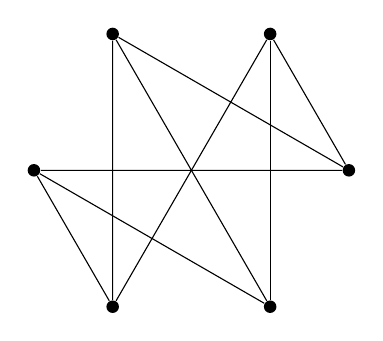
\begin{tikzpicture}
        \node [v] (a1) at (0:2){};
        \node [v] (a2) at (60:2){};
        \node [v] (a3) at (120:2){};
        \node [v] (a4) at (180:2){};
        \node [v] (a5) at (240:2){};
        \node [v] (a6) at (300:2){};
        \draw (a1)--(a2)--(a5)--(a3)--(a1);
        \draw (a1)--(a4)--(a6)--(a3);
        \draw (a2)--(a6);
        \draw (a5)--(a4);
    \end{tikzpicture}
    \qquad
    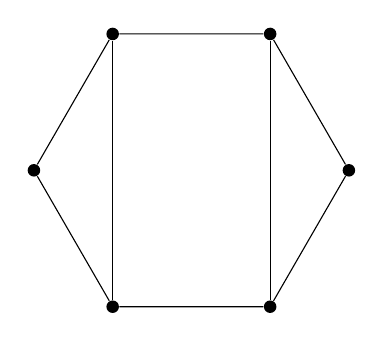
\begin{tikzpicture}
        \node [v] (a1) at (0:2){};
        \node [v] (a2) at (60:2){};
        \node [v] (a3) at (120:2){};
        \node [v] (a4) at (180:2){};
        \node [v] (a5) at (240:2){};
        \node [v] (a6) at (300:2){};
        \draw (a1)--(a2)--(a3)--(a4)--(a5)--(a6)--(a1);
        \draw (a2)--(a6);
        \draw (a3)--(a5);
    \end{tikzpicture}
    \end{center}
    \begin{center}
    \begin{graphfig}{\themycounter\stepcounter{mycounter}}[h]
    \end{graphfig}
    \end{center}\color{red} Missing an edge in the second graph, but yes! \color{black}
We now count the graphs of order 8. Realize that if any vertex is not connected to its diameter, then the path to its diameter will be at least of length 3. \color{red} Not necessarily; there's 2 more possibilities, one with 2 diameters and one with only a single diameter. \color{black} Thus every vertex must be connected to its diameter as follows:
\begin{center}
\begin{graphfig}{\themycounter\stepcounter{mycounter}}
        \gcycle{8}{0.9}{a}
        \draw (a1)--(a2)--(a3)--(a4)--(a5)--(a6)--(a7)--(a8);
        \draw (a1)--(a5) (a2)--(a6) (a3)--(a7) (a4)--(a8);
\end{graphfig}
\end{center}
Thus we have 3 different 3-regular graphs of diameter 2.

\end{proof}

\item Recall that a graph is unipancyclic if it has \textit{exactly} one cycle of length $3$, exactly one cycle of length $4$, etc. 
\begin{enumerate}
    \item Draw a unipancyclic graph of order $3$.
    \begin{center}
    \begin{graphfig}{\themycounter\stepcounter{mycounter}}
        \gcycle{3}{0.9}{a}
    \end{graphfig}
    \end{center}
    \item Draw a unipancyclic graph of order $5$.
    \begin{center}
    \begin{graphfig}{\themycounter\stepcounter{mycounter}}
        \gcycle{5}{0.9}{a}
        \draw (a1)--(a3);
    \end{graphfig}
    \end{center}
    \item Prove there can't be a unipancyclic graph of order 6. 
    \begin{center}
        \begin{graphfig}{}
            \gcycle{6}{0.9}{a}
            \draw (a1)--(a4);
        \end{graphfig}
        \qquad
        \begin{graphfig}{}
            \gcycle{6}{0.9}{a}
            \draw (a1)--(a3) (a4)--(a6);
        \end{graphfig}
    \end{center}
    \begin{center}\begin{graphfig}{\themycounter\stepcounter{mycounter}}\end{graphfig}\end{center}\color{red} Explain what I'm looking at here; these are just two graphs. \color{black}
\end{enumerate}
\item There are seven known unipancyclic graphs : One of order 3, one of order 5, two of order 8, three of order 14. Find them all. 
\begin{center}
    \begin{graphfig}{\themycounter\stepcounter{mycounter}}
        \gcycle{3}{0.9}{a}
    \end{graphfig}
    \qquad
    \begin{graphfig}{\themycounter\stepcounter{mycounter}}
        \gcycle{5}{0.9}{a}
        \draw (a1)--(a3);
    \end{graphfig}
    \qquad
    \begin{graphfig}{\themycounter\stepcounter{mycounter}}
        \gcycle{8}{0.9}{a}
        \draw (a1)--(a3) (a3)--(a7);
    \end{graphfig}
    \qquad
    \begin{graphfig}{\themycounter\stepcounter{mycounter}}
        \gcycle{8}{0.9}{a}
        \draw (a1)--(a3) (a4)--(a7);
    \end{graphfig}
    \qquad
    \begin{graphfig}{\themycounter\stepcounter{mycounter}}
        \gcycle{14}{0.9}{a}
        \draw (a1)--(a3) (a3)--(a6);
    \end{graphfig}
    \qquad
    \begin{graphfig}{\themycounter\stepcounter{mycounter}}
        \gcycle{14}{0.9}{a}
        \draw (a1)--(a3) (a5)--(a8);
    \end{graphfig}
    \qquad
    \begin{graphfig}{\themycounter\stepcounter{mycounter}}
        \gcycle{14}{0.9}{a}
        \draw (a1)--(a3) (a4)--(a7);
    \end{graphfig}
\end{center}\color{red} Good work on order 8! But the order 14 ones don't work; none of them have a 5-cycle. \color{black}
\item We define the complete \textbf{tripartite} graph $K_{a,b,c}$ to be a set of three groups of vertices where there is an edge between every pair of vertices that are in different groups, but no edges between vertices in the same group.
\begin{center}
\begin{graphfig}{\themycounter\stepcounter{mycounter}}
  \node[v] (a1) at (-0.6, 2.8){};
  \node[v] (a2) at ( 0.6, 2.8){};
  \node[v] (b1) at (-3,-0.3){};
  \node[v] (b2) at (-3,-1.4){};
  \node[v] (b3) at (-3,-2.5){};
  \node[v] (c1) at ( 3, 0.2){};
  \node[v] (c2) at ( 3,-0.7){};
  \node[v] (c3) at ( 3,-1.6){};
  \node[v] (c4) at ( 3,-2.5){};
  \foreach \a in {1,2}{\foreach \b in {1,2,3}{\draw[edge] (a\a)--(b\b);}}
  \foreach \a in {1,2}{\foreach \c in {1,2,3,4}{\draw[edge] (a\a)--(c\c);}}
  \foreach \b in {1,2,3}{\foreach \c in {1,2,3,4}{\draw[edge] (b\b)--(c\c);}}
  \node[above=3pt] at (a2) {$A$};
  \node[left=3pt]  at (b1) {$B$};
  \node[right=3pt] at (c1) {$C$};
\end{graphfig}
\end{center}
Find a necessary and sufficient condition for $K_{a,b,c}$ to be Eulerian. 
\begin{proof}
The necessary and sufficient condition for $K_{a,b,c}$ to be an Eulerian graph is that the degree of every vertex must be even. For the degree of each vertex to be even, $a+b$, $b+c$, and $c+a$ must each be even. \color{red} Sure; can you make it any simpler? \color{black}
\end{proof}
\item Show that, in any group of two or more people, there are always at least two who have the same number of friends in the group. 
\begin{proof}
Let there be $n$ people. If we treat each person as a vertex, \color{red} You should also say what edges are! \color{black} the possible degrees are $0, 1, \dots, n-1$, totaling $n$ distinct values. If the degrees of all $n$ people are different, there must be individuals with degrees $0$ and $n-1$ simultaneously. However, a person with degree $n-1$ is connected to everyone else, whereas a person with degree $0$ is connected to no one; this creates a contradiction. Therefore, at least two people must have the same degree. \color{red} Great argument! \color{black}
\end{proof}
\item \textit{CHALLENGE. } Let $T$ be a tree of order $n > 1$. Show that the number of leaves is 
$$ 2 + \sum_{deg(v_i) \geq 3}{(deg(v_i)-2)}$$
Where the sum is over all vertices of degree $3$ or more. 

\item \textit{CHALLENGE. } Compute $R(3,4)$. Btw the answer is 9. 
\item \textit{CHALLENGE. } Find a $4$-regular Harris Graph 



\color{blue} RW: This was a very nice homework assignment! I am glad you introduced me to Overleaf, I quite like this program. Thank you!  \color{black}
\color{green} Very well done overall. Read Zander's comments carefully. Your formatting is obviously amazing, but make sure the math is solid. You all write very well, and some of your proofs had nice creativity to them!\color{black}
\end{enumerate}

\end{document}
